\renewcommand{\arraystretch}{1.5}
\begin{tabular}{| c | c | c | c | c |}
\hline
\begin{tikzpicture}[scale=0.4]
\end{tikzpicture} &
\begin{tikzpicture}[scale=0.4]
  \coordinate[label=above:$a$] (a) at (2,3.464);
  \coordinate[label=above:$b$] (b) at (6,3.464);
  \coordinate[label=below:] (c) at (0,0);
  \coordinate[label=below:] (d) at (4,0);

  \draw[black,fill] (a) circle [radius=0.1cm] ;
  \draw[black,fill] (b) circle [radius=0.1cm] ;
\end{tikzpicture} &
\begin{tikzpicture}[scale=0.4]
  \coordinate[label=above:$a$] (a) at (2,3.464);
  \coordinate[label=above:$b$] (b) at (6,3.464);
  \coordinate[label=below:$c$] (c) at (0,0);
  \coordinate[label=below:$d$] (d) at (4,0);

  \draw (a) -- (b) -- (d);
  \draw[black,fill] (a) circle [radius=0.1cm] ;
  \draw[black,fill] (b) circle [radius=0.1cm] ;
  \draw[black,fill] (c) circle [radius=0.1cm] ;
  \draw[black,fill] (d) circle [radius=0.1cm] ;
\end{tikzpicture} &
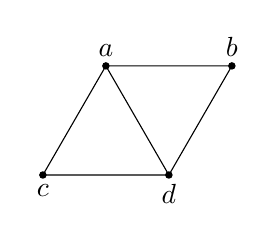
\begin{tikzpicture}[scale=0.4]
  \coordinate[label=above:$a$] (a) at (2,3.464);
  \coordinate[label=above:$b$] (b) at (6,3.464);
  \coordinate[label=below:$c$] (c) at (0,0);
  \coordinate[label=below:$d$] (d) at (4,0);

  \draw (a) -- (d) -- (c) -- cycle;
  \draw (d) -- (b) -- (a);
  \draw[black,fill] (a) circle [radius=0.1cm] ;
  \draw[black,fill] (b) circle [radius=0.1cm] ;
  \draw[black,fill] (c) circle [radius=0.1cm] ;
  \draw[black,fill] (d) circle [radius=0.1cm] ;
\end{tikzpicture} &
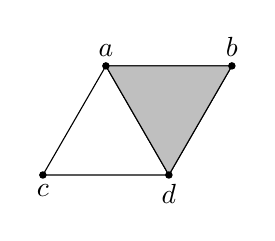
\begin{tikzpicture}[scale=0.4]
  \coordinate[label=above:$a$] (a) at (2,3.464);
  \coordinate[label=above:$b$] (b) at (6,3.464);
  \coordinate[label=below:$c$] (c) at (0,0);
  \coordinate[label=below:$d$] (d) at (4,0);

  \draw (a) -- (d) -- (c) -- cycle;
  \draw (d) -- (b) -- (a);
  \draw[fill=gray!50] (a) -- (d) -- (b) -- cycle;
  \draw[black,fill] (a) circle [radius=0.1cm] ;
  \draw[black,fill] (b) circle [radius=0.1cm] ;
  \draw[black,fill] (c) circle [radius=0.1cm] ;
  \draw[black,fill] (d) circle [radius=0.1cm] ;
\end{tikzpicture} \\
\hline
$\emptyset = K_0$ & $K_1$ & $K_2$ & $K_3$ & $K_4 = K$ \\
\hline
\end{tabular}